\chapter{Drift Chamber 05} \label{ch::DC05}
\subsection{Motivation}
A new drift chamber (DC05) was added for the
2015 Drell-Yan data taking.  This detector was built in collaboration
with UIUC, Abilene Christian University and Old Dominion University.
The author of this prelim paper has made significant contributions to
all the construction, testing, calibration and performance evaluation
of DC05.  From simulations it was determined
that 95\% of all Drell-Yan events include a muon track in LAS.
Therefore the COMPASS trigger system was setup to record Drell-Yan
data only when at least one muon track is included in LAS.
However two large area trackers, straw type detectors, were suffering
from age related temperature effects in LAS.  Simulations also
concluded that the reconstructed track efficiency in LAS reduces to
30\% without the redundancy from one and a half of its large area
trackers.  DC05 was built to replace a straw detectors in LAS to
ensure stable Drell-Yan data taking in 2015 and in the years
following.

\subsection{DC05 Design}

%\begin{figure}[h]
%  \centering 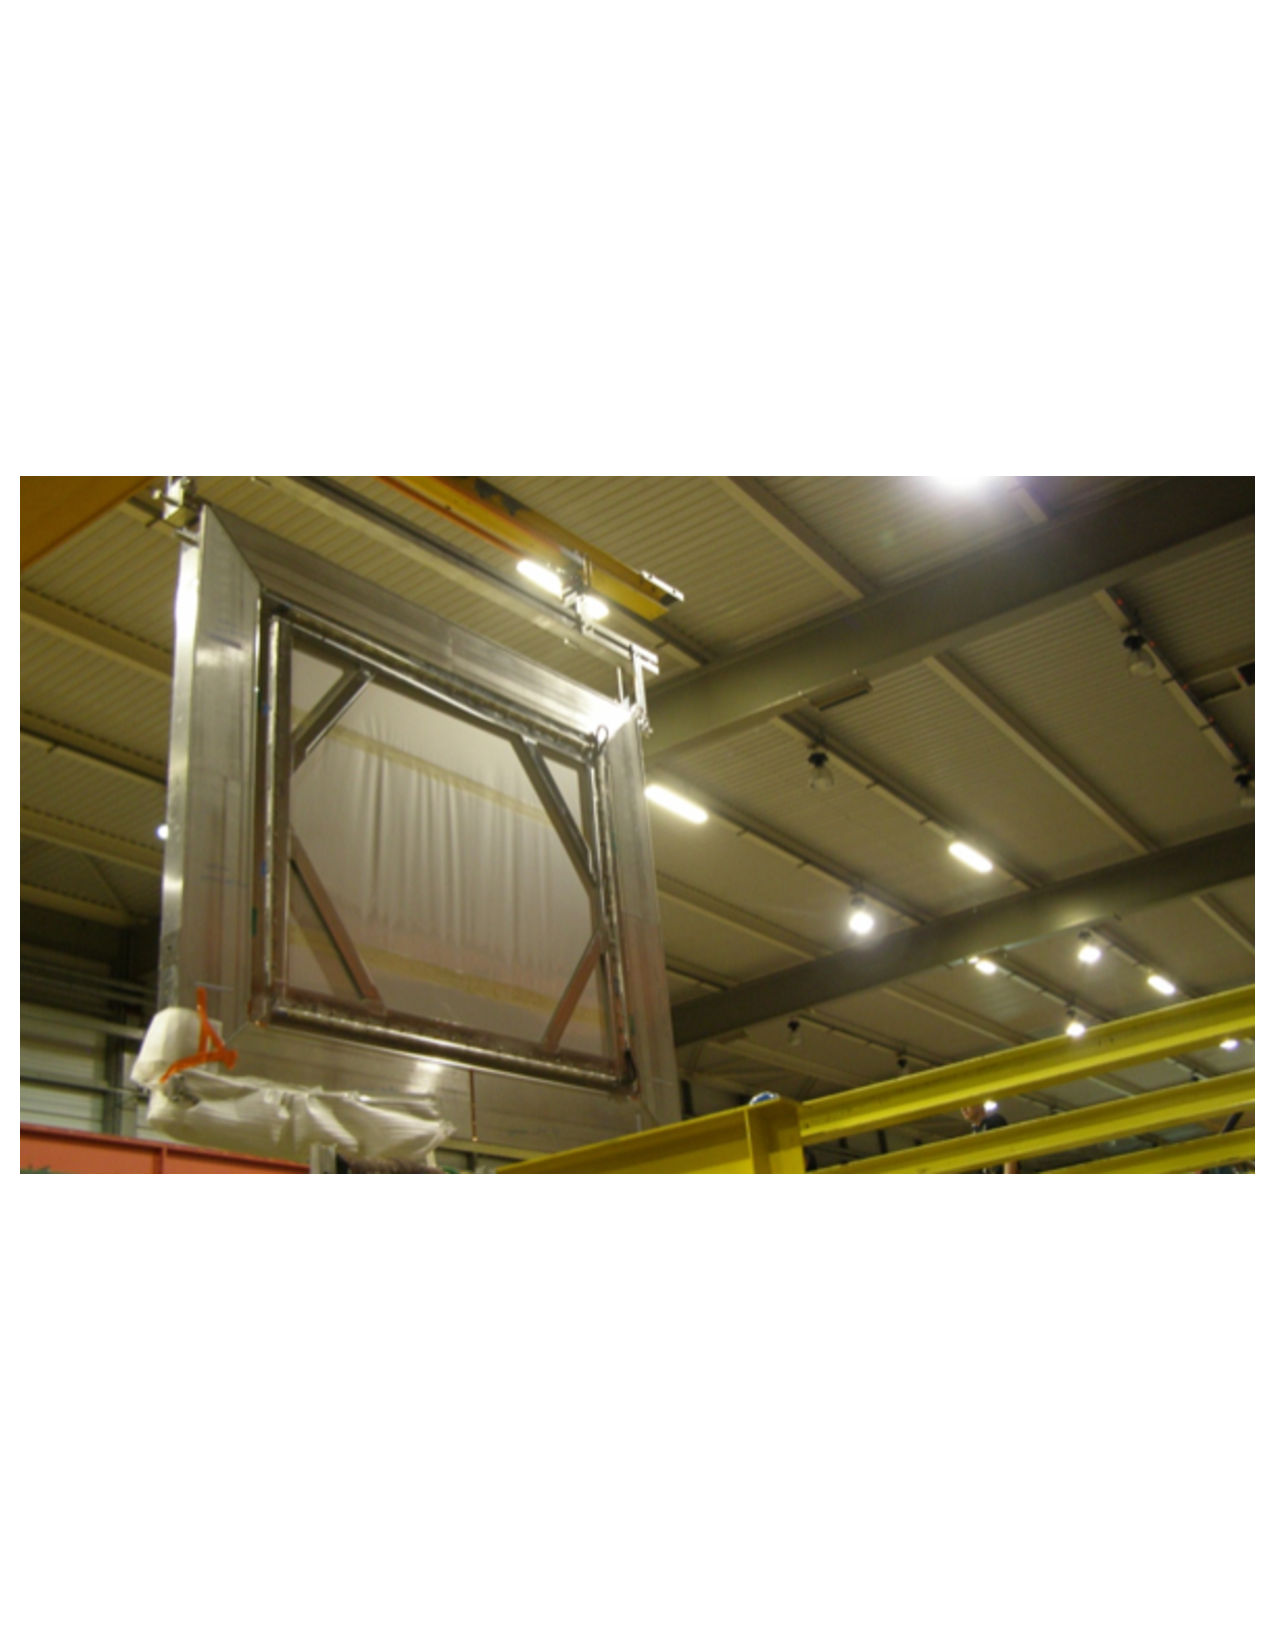
\includegraphics[width=0.5\textwidth]{DC05_full}
%  \caption{}{The completed Drift Chamber 05 being craned into the
%    COMPASS large angle spectrometer in May, 2015.}
%  \label{fig:DC05_full}%
%\end{figure}

The design of DC05, see figure~\ref{fig:DC05_full}, was based off a
previous large-area tracker at COMPASS.  DC05 has an active area of
249x209~cm$^2$ and consists of eight planes with a total of 2304 sense
wires and 2312 field wires.  The eight planes of DC05 measure the X and Y
views and $\pm$ 10$^{\circ}$ with respect to the X coordinates (U/V
views).  The X and Y views each consist of 2x256 sense wires and the
U/V views each consist of 2x320 wires for increased acceptance. The
whole detector was closed in with two precision, stainless steel
stiffening frames which were assembled with aluminized mylar as a gas
window. \par

Each of the four views of DC05 are made from five layers of G-10
frames and consists of three cathode layers and two anode layers.
Additionally a 30~cm circular ``beam killer'' was added to the
cathodes to control the efficiency in the central part of the
detector.  The beam killer was added to be able to prevent pile up effects from
the high beam flux.  The cathodes were nominally set to -1675 V, which
was found to be in the efficiency plateau high voltage region and the
beam killer voltage was set to -900 V for no amplification in the high
flux central region.  Conviently the voltage on the beam killer can
however be adjusted to study the central region during times of low
beam flux such as alignment physics data taking.  \par

%\begin{figure}[h]
%  \centering 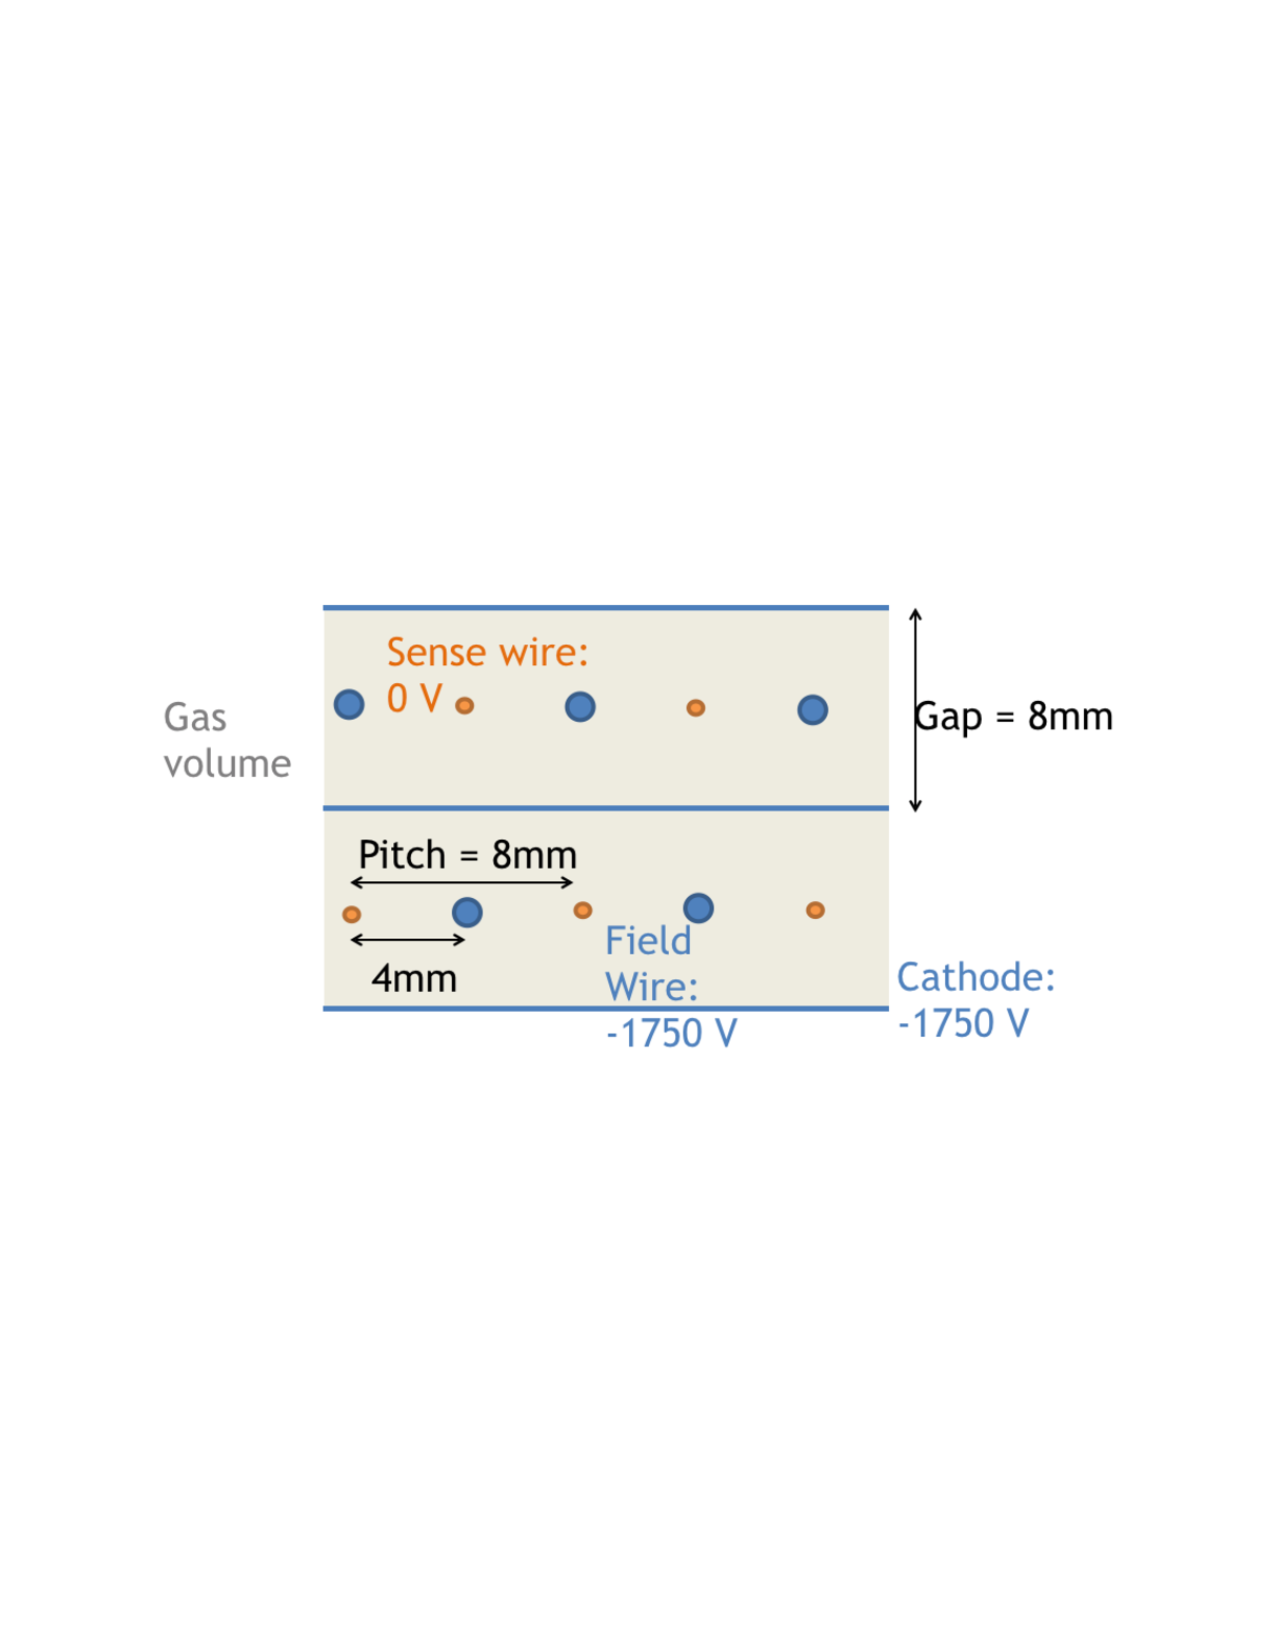
\includegraphics[width=0.45\textwidth]{DriftCell}
%  \caption{}{The drift cell dimensions of one view in Drift Chamber
%    05.}
%  \label{fig:DriftCell}%
%\end{figure}

The anode layers were made from alternating 20~$\mu$m gold-plated
tungsten sense wires and 100~$\mu$m gold-plated copper beryllium field
wires, as shown in figure~\ref{fig:DriftCell}.  The field wires were
also placed at -1675 V and the sense wires were at 0 V.  The gas used
was made of: 45\% argon, for amplification; 45\% ethane, for
quenching; and 10\% CF$_4$, to reduce aging effects.  All these
properties correspond to a gain of approximately 10$^4$.

\subsection{Construction}
The construction of DC05 was built as precise as possible starting
with the precision from the stainless steel stiffening frames.  The
two stiffening frames were cut on top of each other for the highest
relative accuracy and were cut to a precision of 50~$\mu$m everywhere
in their plane.  The precision from the stiffening frames was then
transferred to the anode and cathode frames through 40 positioning
pins.  The G-10 frames were milled from strips at the nuclear physics
lab using a high precision milling machine.  Each four strips were
then epoxied together, forming lap joints at the corners, on top of
one of the stiffening frames for the highest relative accuracy.  \par

The cathodes had 25~$\mu m$ thin mylar stretched and epoxied to them
using a custom-built stretching machine at CERN.  The cathodes layers
then had carbon spray painted on and were hand polished till we
achieved a resistance of approximately 30~$k\Omega$/m.  All the sense
and field wires were hand soldered and subsequently verified for
position using a microscope.  It was estimated the position placement
of each sense wire was at least as good as half the diameter of a
sense wire or precise to 10~$\mu$m.  The final assemble was done at
CERN.  This consisted of stacking each of the 21 G-10 frames on top of
the stiffening frame and attaching copper shielding all along the
exterior of the detector to reduce electronic noise. \par

There were various test performed throughout the construction process
for quality assurance before the final installation.  The starting
tests were measuring thickness and position of important cuts on the
G-10 strips using a micrometer.  G-10 strip thicknesses were
iteratively milled until they reached better than 50~$\mu$m in
thickness accuracy and all 21 G-10 frames plus two stiffening frames
stacked together were around 700~$\mu$m in thickness accuracy.  The
mechanical tension of the sense wires was tested for stability by
ensuring the voltage difference between sense and field wires could
reach as high as 2400 V in air and cross checked by determining the
frequency with which the wires vibrated.  The leakage current between
sense and field wires was verified to be less than 100 nA at nominal
voltage in air.  Finally amplification tests were first performed
using a strontium-90 source and verifying the counts per electronics
board increased at the appropriate locations.

\subsection{DC05 Calibration}

%\begin{figure}[h]
%  %\centering 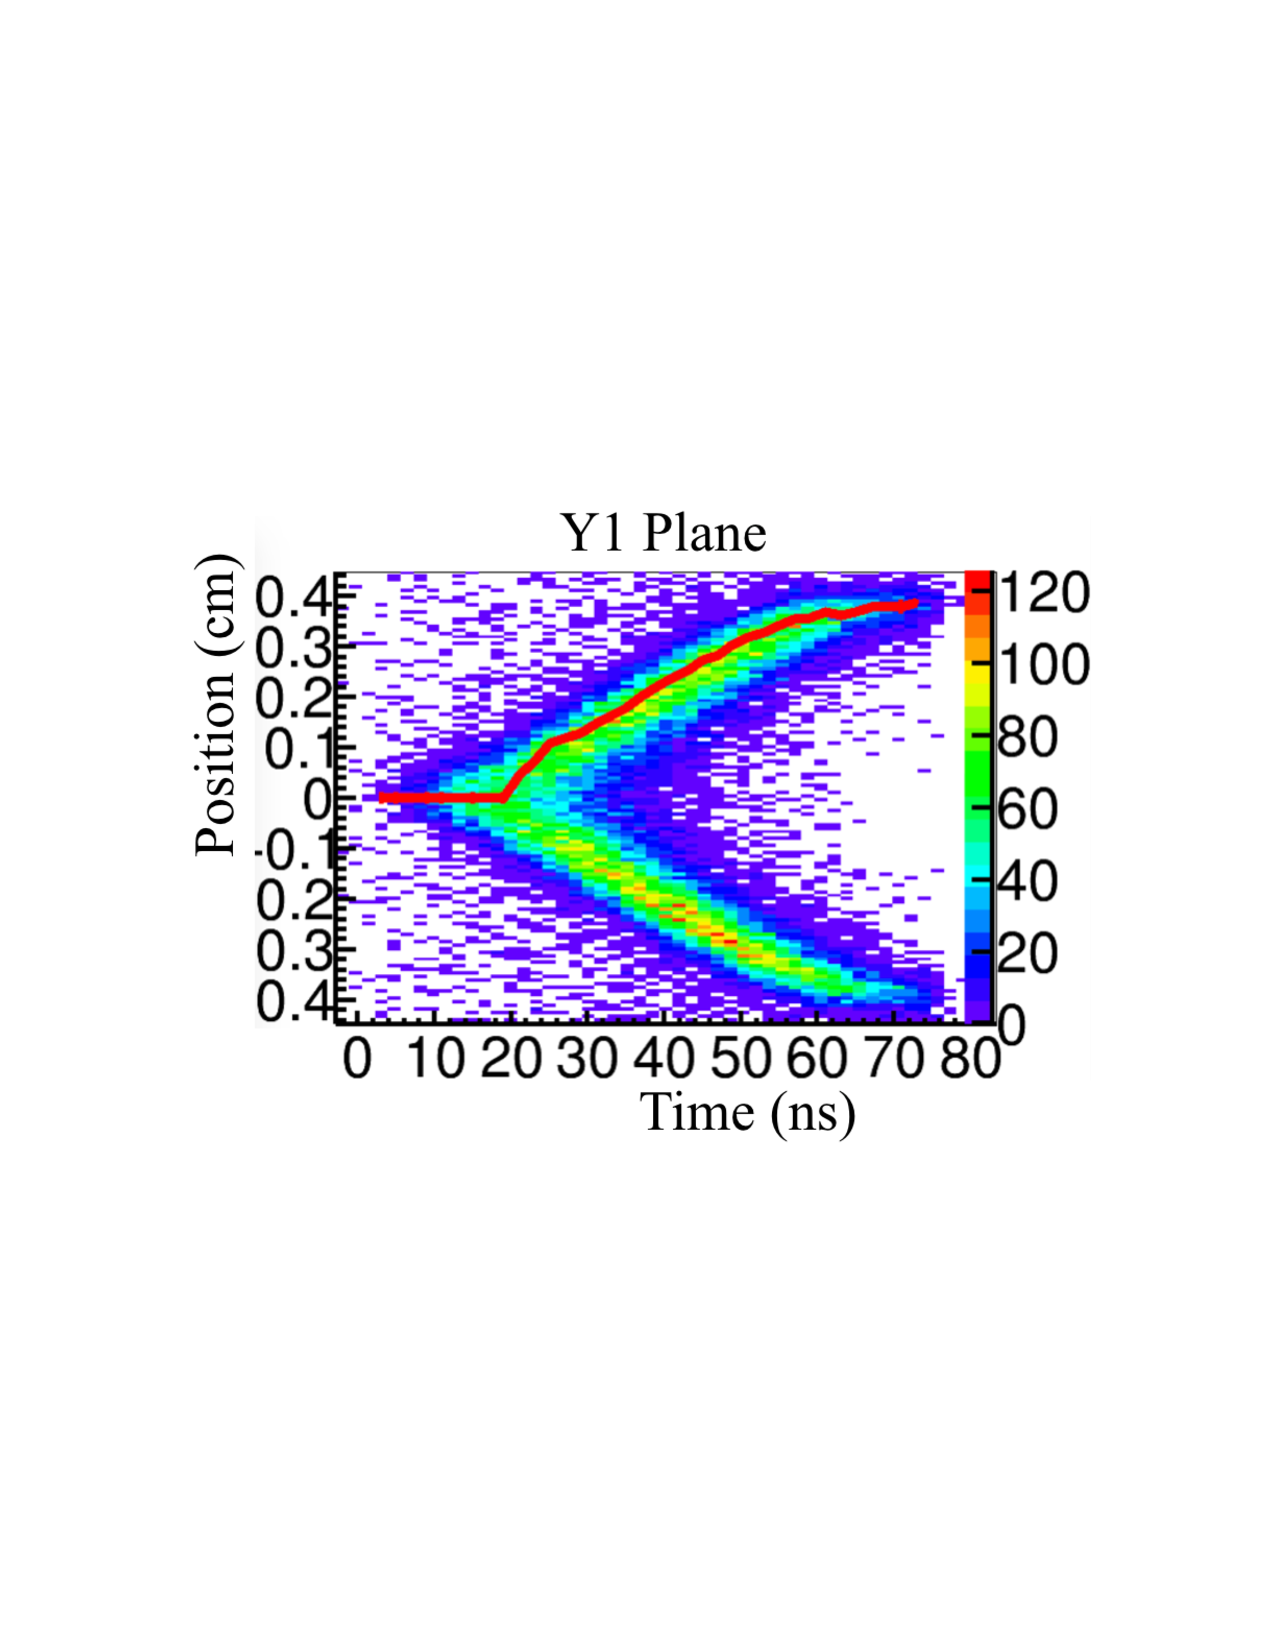
\includegraphics[width=0.5\textwidth]{RT_DC05Y2.png}
%  \centering 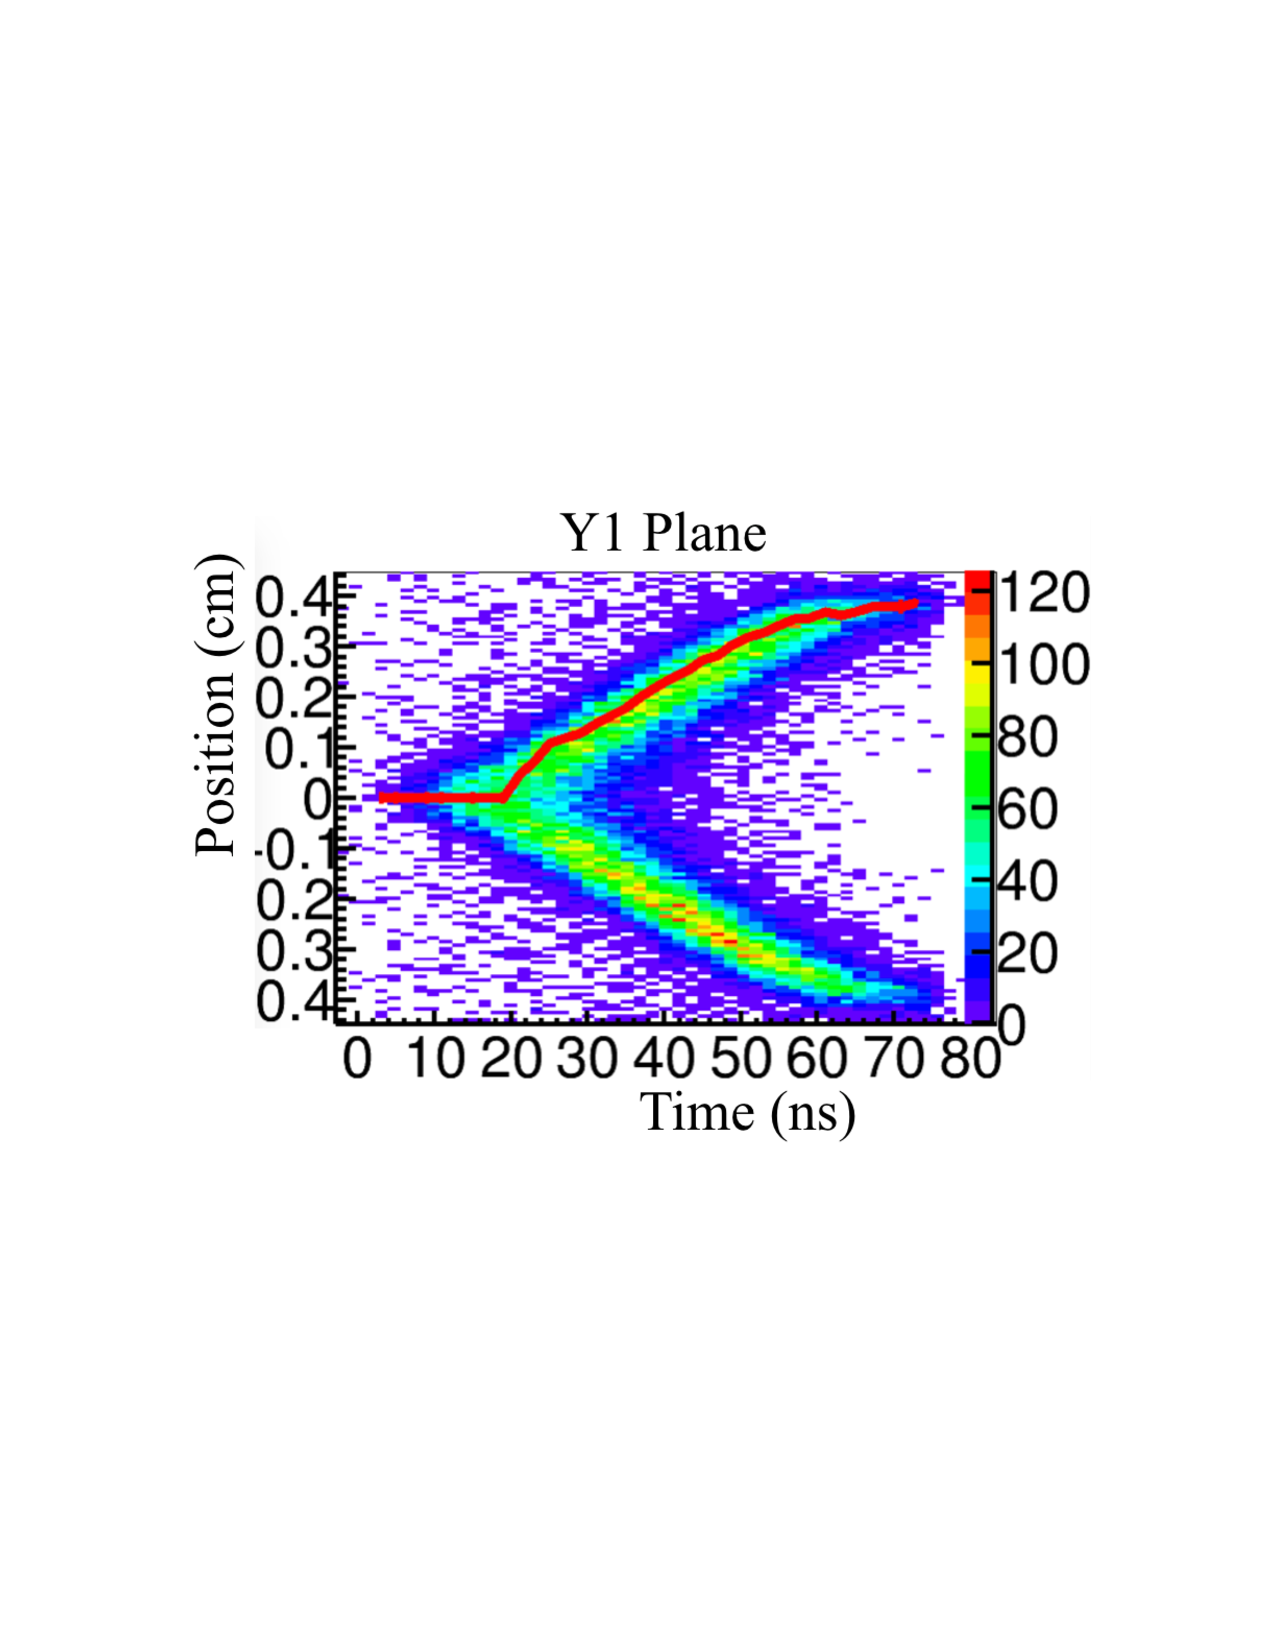
\includegraphics[width=0.45\textwidth]{RT_DC05Y2.png}
%  \caption{}{Time versus position relation, RT relation, after
%    calibrating.  The red line shows the calibration determined.}
%  \label{fig:RT_DC05Y2}%
%\end{figure}

%\begin{figure}[h]
%  \centering
%  \begin{subfigure}{0.47\textwidth}
%    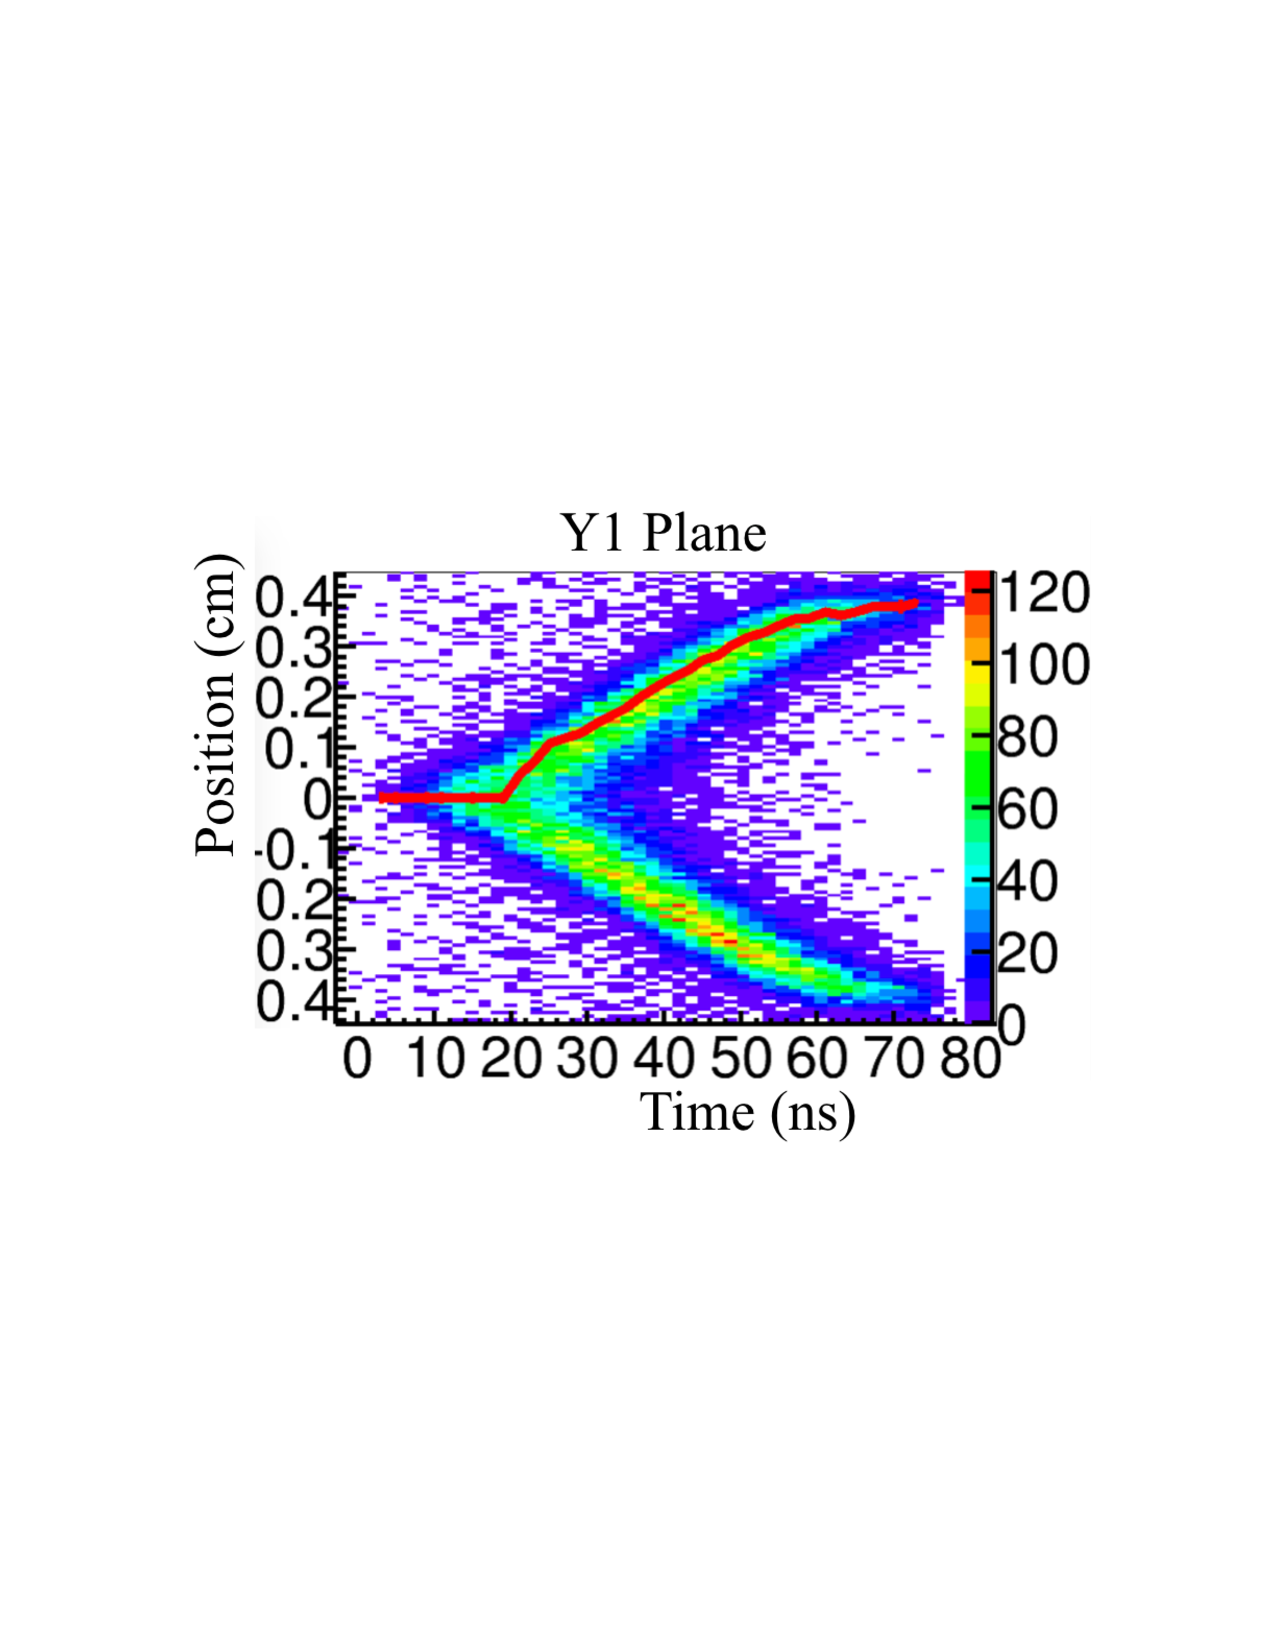
\includegraphics[width=1.0\textwidth]{RT_DC05Y2.png}
%    \caption{}{Time versus position relation, RT relation, after
%      calibrating.  The red line shows the calibration determined.}
%    \label{fig:RT_DC05Y2}%
%  \end{subfigure}
%  \begin{subfigure}{0.47\textwidth}
%    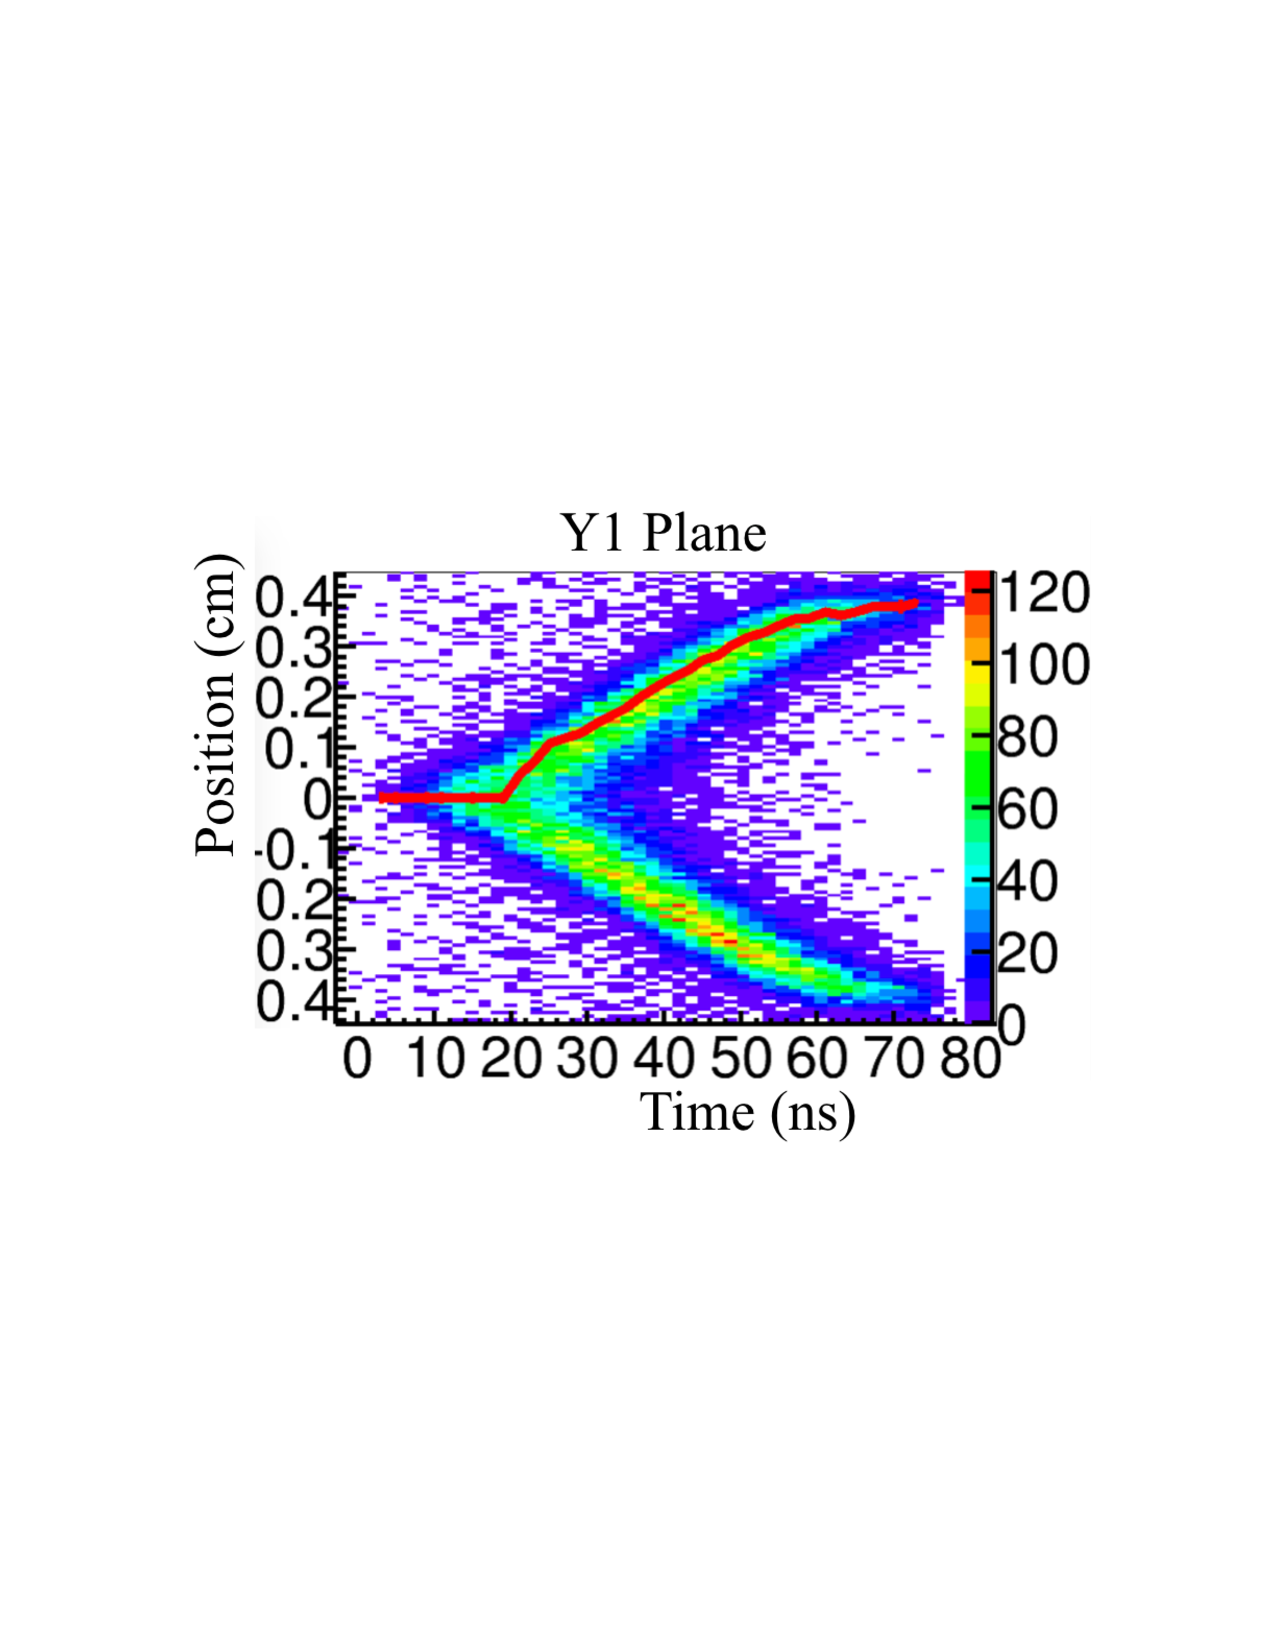
\includegraphics[width=1.0\textwidth]{RT_DC05Y2.png}
%    \caption{}{To be changed later.}
%    \label{fig:tmp}%
%  \end{subfigure}
%\end{figure}

The detector was calibrated using a position as a function of time
plot, the so called RT relation.  An example of the RT relation is
shown in figure~\ref{fig:RT_DC05Y2} where the position is the location of
a track, within a drift cell, relative to the center sense wire and the 
time used is DC05's timing relative to the trigger time.  The calibration was performed,
using a plot like figure~\ref{fig:RT_DC05Y2}, by taking y-projection
slices and finding the peaks of the upper half of the RT curve where the
red curve on figure~\ref{fig:RT_DC05Y2} shows an example of the found
calibration curve.  Only a positive position relation is defined
because it is assumed that the upper and lower portions of the RT
relations are symmetric and that a positive or negative distance is
resolved by having two planes measure the same coordinate but offset
by half a drift cell.  The ability to make an RT relation is what sets
drift chambers apart from proportional counters by allowing the
determination of a charged particle's position within a drift cell.
This allows drift chambers to have a better position resolution.

\subsection{2015 DC05 Performance}
The overall performance of DC05 was checked using the CORAL
reconstruction software of COMPASS.  In all cases the view of study
was excluded from the reconstruction algorithm and the individual hit
information for the view of interest was saved to get an unbiased
measurement. \par

The efficiency was found by opening a road of 1.2 mm radius around the
expected track location and determining if the DC05 plane of interest
received a hit in this area or not.  To ensure the best position
resolution of the track selection and to prevent ghost tracks, the
selected tracks were required to come from a primary vertex in the
target.  In 2015 DC05 was found to have an efficiency between 85\% and
90\% depending on the plane.  Some results of the 1-dimensional and
2-dimensional computed efficiency are shown in
figure~\ref{fig:DC05_efficiency}. \par

%, where the central and band leading
%up to the center inefficient zones were dead zones due to the beam
%killer. \par

%\begin{figure}[h]
%  \centering \includegraphics[width=0.7\textwidth]{DC05_efficiency}
%  \caption{The 1-dimensional and 2-dimensional efficiencies of the
%    Y-planes in DC05.}
%  \label{fig:DC05_efficiency}
%\end{figure}

The resolution of DC05 was determined from the double layer residual.
The double layer residual is the measured difference between upstream
residual and the downstream residual of a coordinate view.  This
double-layer residual is independent of the track resolution and only
depends on the variance addition of the two individual planes.  The
same track selection for efficiency determination was also used for
position resolution determination.  For the 2015 Drell-Yan physics
taking the resolution achieved was approximately 430~$\mu$m.  We determined
this by fitting the double residual with a Gaussian to extract the
variance and assumed equal variance per plane in a view.
